\subsubsection*{Informazioni sul package}
\begin{figure}[h]
	\centering
	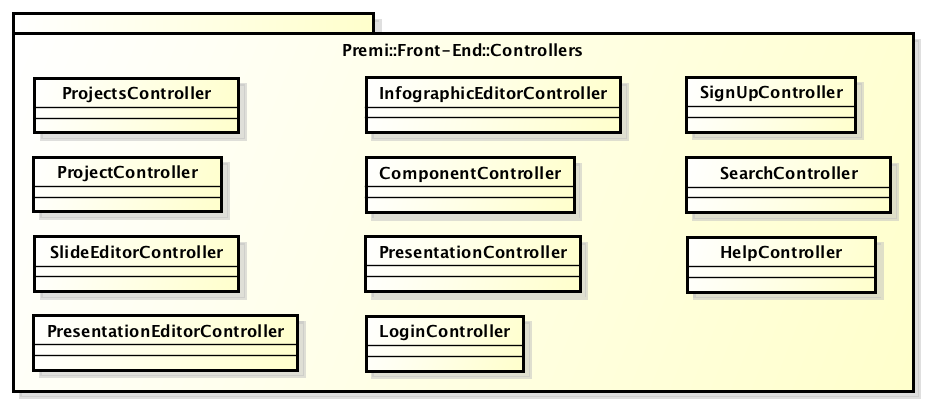
\includegraphics[width=1.0\linewidth]{img/front-end_controllers}
	\caption[Premi::Front-End::Controllers]{Premi::Front-End::Controllers}
\end{figure}
\begin{itemize}
	\item \textbf{Descrizione}: Il package serve a far comunicare le view con il model in entrambe le direzioni ovvero rendere visibili gli aggiornamenti del model nella view e viceversa aggiornare il model con le informazioni provenienti dalla view.
	\item \textbf{Interazione con altri package}:
	\begin{itemize}
		\item Vi è un'interazione con il package Premi::Front-End::Views in quanto i controller sono utilizzati per iniziallizzare le view e per aggiornare il model del frontend con le modifiche avvenute in esse;
		\item Vi è un'interazione con il package Premi::Front-End::Model poiché in esso vengono depositati e prelevati i dati necessari alle view richieste;
		\item Vi è un'interazione con il package Premi::Front-End::Services responsabile del recupero e salvataggio delle informazioni e dell'invocazione di precise procedure dall'esterno mediante chiamate REST.
	\end{itemize}

\end{itemize}

\subsubsection*{Classi contenute}
\begin{itemize}

	\item Premi::Front-End::Controllers::ProjectsCtrl:
	\begin{itemize}
		\item \textbf{Descrizione}: classe con lo scopo di fornire le operazioni necessarie alla visualizzazione e gestione dei progetti relativi ad un utente.
		\item \textbf{Relazioni con altre classi}:
		\begin{itemize}
			\item Premi::Front-End::Services::ProjectService;
			\item Premi::Front-End::Views::Projects.
		\end{itemize}
	\end{itemize}
	\item  Premi::Front-End::Controllers::ProjectCtrl:
	\begin{itemize}
		\item \textbf{Descrizione}: classe con lo scopo di fornire le operazioni necessarie alla gestione di un progetto.
		\item \textbf{Relazioni con altre classi}:
		\begin{itemize}
			\item Premi::Front-End::Services::ProjectService;
			\item Premi::Front-End::Views::Project.
		\end{itemize}
	\end{itemize}
	\item  Premi::Front-End::Controllers::SlideEditorCtrl:
	\begin{itemize}
		\item \textbf{Descrizione}: classe di suporto all'editor di una presentazione fornendo le operazioni necessarie alla composizione e modifica di una slide. Essa permette di assemblare e modificare una \gls{slide} e i metodi che effettueranno le operazioni sui componenti.
		\item \textbf{Relazioni con altre classi}:
		\begin{itemize}
			\item Premi::Front-End::Views::SlideEditor;
			\item Premi::Front-End::Controllers::PresentationEditorCtrl;
			\item Premi::Front-End::Services::SlideService;
			\item Premi::Front-End::Controllers::ComponentCtrl;
			\item Premi::Front-End::Controllers::ChartCtrl;
			\item Premi::Front-End::Controllers::ImageCtrl;
			\item Premi::Front-End::Controllers::RealTimeDataCtrl;
			\item Premi::Front-End::Controllers::TableCtrl;
			\item Premi::Front-End::Controllers::TextCtrl.
		\end{itemize}
	\end{itemize}
	\item  Premi::Front-End::Controllers::PresentationEditorCtrl:
	\begin{itemize}
		\item \textbf{Descrizione}: classe con lo scopo di fornire le operazioni necessarie alla gestione dell'editor di una presentazione. Essa permette di assemblare e modificare una \gls{slide} e i metodi che effettueranno le operazioni sui componenti.
		\item \textbf{Relazioni con altre classi}:
		\begin{itemize}
			\item Premi::Front-End::Services::PresentationService;
			\item Premi::Front-End::Views::Presentation;
			\item Premi::Front-End::Controllers::SlideEditorCtrl.
		\end{itemize}
	\end{itemize}
	\item  Premi::Front-End::Controllers::InfographicEditorCtrl:
	\begin{itemize}
		\item \textbf{Descrizione}: classe con lo scopo di fornire le operazioni necessarie alla gestione dell'editor di una inforgrafica. Essa permette di assemblare e modificare una \gls{slide} e i metodi che effettueranno le operazioni sui componenti.
		\item \textbf{Relazioni con altre classi}:
		\begin{itemize}
			\item Premi::Front-End::Services::InfographicService;
			\item Premi::Front-End::Views::InfographicEditor.
		\end{itemize}
	\end{itemize}
	\item  Premi::Front-End::Controllers::ComponentCtrl:
	\begin{itemize}
		\item \textbf{Descrizione}: classe con lo scopo di fornire le operazioni necessarie alla gestione di un componente di una \gls{slide}.
		\item \textbf{Relazioni con altre classi}:
			\begin{itemize}
				\item Premi::Front-End::Model::Component;
				\item Premi::Front-End::Controllers::ChartCtrl;
				\item Premi::Front-End::Controllers::ImageCtrl;
				\item Premi::Front-End::Controllers::RealTimeDataCtrl;
				\item Premi::Front-End::Controllers::TableCtrl;
				\item Premi::Front-End::Controllers::TextCtrl.
			\end{itemize}
	\end{itemize}
	
	
	
	
	
	
	
	
	
	
	
	
	
	
	\item  Premi::Front-End::Controllers::ChartCtrl:
		\begin{itemize}
			\item \textbf{Descrizione}: classe con lo scopo di fornire le operazioni necessarie alla gestione di un grafico.
			\item \textbf{Relazioni con altre classi}:
				\begin{itemize}
					\item Premi::Front-End::Model::Component;
					\item Premi::Front-End::Model::Chart;
					\item Premi::Front-End::Controllers::ComponentCtrl;
					\item Premi::Front-End::Controllers::SlideEditorCtrl;
					\item Premi::Front-End::Services::ChartService.
				\end{itemize}
		\end{itemize}
		
	\item  Premi::Front-End::Controllers::ImageCtrl:
			\begin{itemize}
				\item \textbf{Descrizione}: classe con lo scopo di fornire le operazioni necessarie alla gestione di una immagine.
				\item \textbf{Relazioni con altre classi}:
					\begin{itemize}
						\item Premi::Front-End::Model::Component;
						\item Premi::Front-End::Model::Image;
						\item Premi::Front-End::Controllers::ComponentCtrl;
						\item Premi::Front-End::Controllers::SlideEditorCtrl;
						\item Premi::Front-End::Services::ImageService.
					\end{itemize}
			\end{itemize}
			
	\item  Premi::Front-End::Controllers::RealTimeDataCtrl:
			\begin{itemize}
				\item \textbf{Descrizione}: classe con lo scopo di fornire le operazioni necessarie alla gestione di un componente con aggiornamento in tempo reale.
				\item \textbf{Relazioni con altre classi}:
					\begin{itemize}
						\item Premi::Front-End::Model::Component;
						\item Premi::Front-End::Model::RealTimeData;
						\item Premi::Front-End::Controllers::ComponentCtrl;
						\item Premi::Front-End::Controllers::SlideEditorCtrl;
						\item Premi::Front-End::Services::RealTimeDataService.
					\end{itemize}
			\end{itemize}
			
	\item  Premi::Front-End::Controllers::TableCtrl:
			\begin{itemize}
				\item \textbf{Descrizione}: classe con lo scopo di fornire le operazioni necessarie alla gestione di una tabella.
				\item \textbf{Relazioni con altre classi}:
					\begin{itemize}
						\item Premi::Front-End::Model::Component;
						\item Premi::Front-End::Model::TableCtrl;
						\item Premi::Front-End::Controllers::ComponentCtrl;
						\item Premi::Front-End::Controllers::SlideEditorCtrl;
						\item Premi::Front-End::Services::TableService.
					\end{itemize}
			\end{itemize}
			
	\item  Premi::Front-End::Controllers::TextCtrl:
			\begin{itemize}
				\item \textbf{Descrizione}: classe con lo scopo di fornire le operazioni necessarie alla gestione di un componente di tipo testuale.
				\item \textbf{Relazioni con altre classi}:
					\begin{itemize}
						\item Premi::Front-End::Model::Component;
						\item Premi::Front-End::Model::TextCtrl;
						\item Premi::Front-End::Controllers::ComponentCtrl;
						\item Premi::Front-End::Controllers::SlideEditorCtrl;
						\item Premi::Front-End::Services::TextService.
					\end{itemize}
			\end{itemize}
	
	
	
	
	
	
	
	
	
	
	
	
	
	
	
	\item  Premi::Front-End::Controllers::PresentationCtrl:
	\begin{itemize}
		\item \textbf{Descrizione}: classe con lo scopo di fornire le operazioni necessarie alla gestione della visualizzazione di una presentazione. Essa permette di assemblare e configurare una presentazione e di rendere disponibile la visualizzazione in modalità classica o presentatore.
		\item \textbf{Relazioni con altre classi}:
		\begin{itemize}
			\item Premi::Front-End::Services::PresentationService;
			\item Premi::Front-End::Views::Presentation.
		\end{itemize}
	\end{itemize}
	\item  Premi::Front-End::Controllers::AuthenticationCtrl
		\begin{itemize}
		\item \textbf{Descrizione}: classe con lo scopo di fornire le operazioni necessarie all'autenticazione nel sistema, registrazione,accredito e recupero password di un utente.
		\item \textbf{Relazioni con altre classi}:
		\begin{itemize}
			\item Premi::Front-End::Services::AuthenticationService;
			\item Premi::Front-End::Views::InfographicEditor;
			\item Premi::Front-End::Views::PresentationEditor;
			\item Premi::Front-End::Views::SignUpEditor;
			\item Premi::Front-End::Views::LogIn;
			\item Premi::Front-End::Views::Project;
			\item Premi::Front-End::Model::User.
		\end{itemize}
	\end{itemize}
	\item  Premi::Front-End::Controllers::HomePageCtrl:
	\begin{itemize}
		\item \textbf{Descrizione}: classe con lo scopo di fornire le operazioni necessarie al corretto funzionamento della Home Page. In particolare si occupa della gestione delle funzionalità di ricerca di progetti e presentazioni mediante il titolo oppure il nome dell'utente proprietario.
		\begin{itemize}
			\item Premi::Front-End::Services::ProjectService;
			\item Premi::Front-End::Views::HomePage.
		\end{itemize}
	\end{itemize}
	\item  Premi::Front-End::Controllers::HelpCtrl:
	\begin{itemize}
		\item \textbf{Descrizione}: 
			classe con lo scopo di fornire le operazioni necessarie alla gestione dell'aiuto agli utenti sottoforma di tour\footnote{Un tour è una esplorazione guidata delle funzionalità basilari del sistema al fine di permettere all'utente di familiarizzare velocemente con esso.} e suggerimenti.
		\item \textbf{Relazioni con altre classi}:
			\begin{itemize}
				\item Premi::Front-End::Views::SlideEditor;
				\item Premi::Front-End::Views::InfographicEditor;
				\item Premi::Front-End::Views::Projects;
				\item Premi::Front-End::Views::Search.
			\end{itemize}
			
	\end{itemize}
	\item  Premi::Front-End::Controllers::MyAccountCtrl:
		\begin{itemize}
			\item \textbf{Descrizione}: 
				classe con lo scopo di fornire le operazioni necessarie alla visualizzazione e gestione del profilo di un utente che si è autenticato nel sistema.
			\item \textbf{Relazioni con altre classi}:	
			\begin{itemize}
				\item Premi::Front-End::Services::AuthenticationService::UserService.
				\item Premi::Front-End::Views::MyAccount.
			\end{itemize}
		\end{itemize}
\end{itemize}
\newpage
